\documentclass[fleqn]{article}
\usepackage[nodisplayskipstretch]{setspace}
\usepackage{amsmath, nccmath, bm}
\usepackage{amssymb}
\usepackage{enumitem}
\usepackage{etoolbox}
\usepackage{graphicx}
\usepackage{float}
\usepackage{changepage}
\usepackage{environ,capt-of}

\let\oldfigure\figure% Store original figure float environment
\let\endoldfigure\endfigure
\RenewEnviron{figure}[1][H]{% Update figure environment
  %\par\vspace{\intextsep}% Assume in-text placement, so insert appropriate vertical spacing
  \noindent
  % \patchcmd{<cmd>}{<search>}{<replace>}{<success>}{<failure>}
  \patchcmd{\BODY}{\caption}{\captionof{figure}}{}{}% Replace \caption with \captionof{figure} inside \BODY
  % Set "figure"
  \begin{minipage}{\linewidth}
    \BODY
  \end{minipage}
  %\par\vspace{\intextsep}% Assume in-text placement, so insert appropriate vertical spacing
}

\newcommand{\zerodisplayskip}{
	\setlength{\abovedisplayskip}{0pt}%
	\setlength{\belowdisplayskip}{0pt}%
	\setlength{\abovedisplayshortskip}{0pt}%
	\setlength{\belowdisplayshortskip}{0pt}%
	\setlength{\mathindent}{0pt}}
	
\title{Homework 3}
\author{Owen Sowatzke}
\date{March 13, 2024}

\begin{document}

	\offinterlineskip
	\setlength{\lineskip}{12pt}
	\zerodisplayskip
	\maketitle
	
	\begin{enumerate}
		\item The exclusive-OR is the simplest problem that cannot be solved using a linear discriminant operating directly on the features. The points $k=1,3$ at $\mathbf{x} = [1,1]^T$ and $[-1,-1]^T$ are in the category $\omega_1$ (red in the figure), while $k=2,4$ at $\mathbf{x}=[1,-1]^T$ and $[-1,1]^T$ are in $\omega_2$ (black in the figure). Following the approach of Support Vector Machines, we preprocess the features to map them to a higher dimension space where they can be linearly separated. While many $\varphi$-functions could be used, here we use the simplest expansion up to second order: $1, \sqrt{2}x_1, \sqrt{2}x_2, \sqrt{2}x_1x_2, x_1^2$ and $x_2^2$, where the $\sqrt{2}$ is convenient for normalization. Using the support vector machine formulation, show that the optimum discriminant is $g(\mathbf{x}) = g(x_1,x_2) = x_1 * x_2$.
		
	\begin{figure}[H]
		\centerline{\fbox{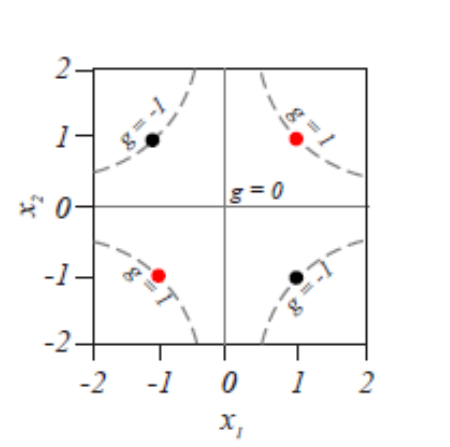
\includegraphics[width=0.4\textwidth]{exclusive_or.png}}}
		\caption{Exclusive-OR Problem}
		\label{exclusive_or}
	\end{figure}
		
	First, we transform the data using the $\varphi$ functions. The resulting data is given as follows:
	
	$\mathbf{x_1} = \varphi(\mathbf{x_1}) = [1,\sqrt{2},\sqrt{2},\sqrt{2},1,1]^T$
	
	$\mathbf{x_2} = \varphi(\mathbf{x_2}) = [1,-\sqrt{2},-\sqrt{2},\sqrt{2},1,1]^T$
	
	$\mathbf{x_3} = \varphi(\mathbf{x_3}) = [1,\sqrt{2},-\sqrt{2},-\sqrt{2},1,1]^T$
	
	$\mathbf{x_4} = \varphi(\mathbf{x_4}) = [1,-\sqrt{2},\sqrt{2},-\sqrt{2},1,1]^T$
	
	Next, we can re-express the problem in a form suitable for quadratic programming. Quadratic programming can be used to find $\mathbf{x}$ which minimizes \newline $\frac{1}{2}\mathbf{x}^T\mathbf{H}\mathbf{x} + \mathbf{f}^T\mathbf{x}$ subject to $\mathbf{Ax} = \mathbf{b}$ and $\mathbf{x} \geq \mathbf{0}$.
	
	Note that we are trying to maximize:
	
	$\mathbf{Q(\boldsymbol{\alpha})} = \sum{a_i} - \frac{1}{2}\sum{\sum{\alpha_i\alpha_jy_iy_j\mathbf{x_i}^T\mathbf{x_j}}}$.
	
	subject to $\sum{a_iy_i} = 0$ and $\alpha_i > 0\ \forall\ i$.
	
	Because the function is quadratic, this is equivalent to minimizing:
	
	$-\mathbf{Q(\boldsymbol{\alpha})} = \frac{1}{2}\sum{\sum{\alpha_i\alpha_jy_iy_j\mathbf{x_i}^T\mathbf{x_j}}} - \sum{a_i}$
	
	Let $\mathbf{\hat{x}_i} = y_i\mathbf{x_i}$ (i.e. let $\mathbf{\hat{x}_i} = \mathbf{x_i}$ for class 1 and let $\mathbf{\hat{x}_i} = -\mathbf{x_i}$ for class 2).
	
	The nested sum can now be written as $\boldsymbol{\alpha}^T\mathbf{\hat{X}}^T\mathbf{\hat{X}}\boldsymbol{\alpha} = \boldsymbol{\alpha}^T\mathbf{H}\boldsymbol{\alpha}$ \newline where $\boldsymbol{\alpha} = [\alpha_1,\alpha_2,\alpha_3,\alpha_4]^T$ and $\mathbf{\hat{X}} = [\mathbf{\hat{x}_1},\mathbf{\hat{x}_2}, \mathbf{\hat{x}_3}, \mathbf{\hat{x}_4}]$.
	
	$-\sum{\alpha_i}$ can also be rewritten as $\mathbf{f}\boldsymbol{\alpha}$ with $\mathbf{f} = [-1,-1,-1,-1]^T$.
	  
	Furthermore, $\sum{\alpha_iy_i} = 0$ is equivalent to $\mathbf{A}\boldsymbol{\alpha} = \mathbf{b}$ where \newline $\mathbf{A} = [y_1,y_2,y_3,y_4] = [1,1,-1,-1]$ and $\mathbf{b} = 0$.
	
	Therefore, we can solve for $\boldsymbol{\alpha}$ which minimizes $\frac{1}{2}\boldsymbol{\alpha}^T\mathbf{H}\boldsymbol{\alpha} + \mathbf{f}^T\boldsymbol{\alpha}$ subject to $\mathbf{A}\boldsymbol{\alpha} = \mathbf{b}$ and $\boldsymbol{\alpha} \geq 0$, where $\mathbf{H}$, $\mathbf{f}$, $\mathbf{A}$, and $\mathbf{b}$ are given above.
	
	Doing so results in the following weight vector:
	
	\begin{equation*}
		\boldsymbol{\alpha} = [1/8,1/8,1/8,1/8]^T
	\end{equation*}
	
	Now, we can solve for $\mathbf{w}$ as follows:
	
	$\mathbf{w} = \sum{\alpha_iy_i\mathbf{x_i}} = \boldsymbol{\hat{X}}\boldsymbol{\alpha} = [0,0,0,1/\sqrt{2},0,0]^T$
	
	Finally, we can solve for $\mathbf{b}$ as follows:
	
	$\mathbf{b} = y_1 - \mathbf{w}^T\mathbf{x_1} = 1 - 1 = 0$
	
	The optimal discriminant $g(x_1,x_2)$ is then given as follows:
	
	$g(x_1,x_2) = \mathbf{w}^T\mathbf{x} + b = \frac{1}{\sqrt{2}}(\sqrt{2}x_1x_2) + 0 = x_1x_2$.
	
	\item Consider a Support Vector Machine and the following training data from two categories:
	
	\begin{center}
	\begin{tabular}{| c | c | c |}
		\hline
		category & $x_1$ & $x_2$ \\
		\hline
		$\omega_1$ & $1$ & $1$ \\
		$\omega_1$ & $2$ & $2$ \\
		$\omega_1$ & $2$ & $0$ \\
		\hline
		$\omega_2$ & $0$ & $0$ \\
		$\omega_2$ & $1$ & $0$ \\
		$\omega_2$ & $0$ & $1$ \\
		\hline
	\end{tabular}
	\end{center}
	
	\begin{enumerate}
		\item[(a)] Plot these six training points, and construct by inspection the weight vector for the optimal hyperplane, and the optimal margin.
		
		\item[(b)] What are the support vectors?
		
		\item[(c)] Construct the solution in the dual space by finding the Lagrange undetermined multipliers, $\alpha_i$. Compare your result to that in \newline part (a).
	\end{enumerate}
	\end{enumerate}
\end{document}